\chapter{Concept implemented}
As per the requirements given by the BMW, idea is to implement a User-Interface which can be used to play the recorded rosbag with more clarification and detailed information display of some ros-topics which were required for understanding the errors and failure. This implementation is based on the idea of webviz tool, where the required rosbag is uploaded to the website and rosbag is played in that tool.

So in this project the approach was to send the HTML requests from the frontend webpage. The backend side will work with the ROS service call and topic. The communication protocol required between the frontend side and ROS will happen via websockets and rosbridge. In this project some of the functionalities like uploading of the rosbag to the cloud, getting information from the rosbag, for updating the information of environments of the factory is done using the REST-API tool.  

Basically playing the rosbag is considered as playing the video on video player. So the requirements were framed using that idea. The basic idea was to upload the bagfile to the cloud. Then we will select the bagfile to be analysed. This bagfile should be loaded in the backend using the ros-tools. Once the bagfile is loaded we must be able to play, pause and play the bagfile as many times, we must be able to step to the particular time in the rosbag using the slider. On the other we must also be able to manipulate the playback speed of the rosbag such that we can play with the required speed. 

Here as the rosbag is recorded in the different factories of the BMW, so map of factories will change. Since with the rosbag record we cannot take the map, so selecting of environments should be enabled. 

In BMW factories, movement of materials happens with str. Since they use different versions of str, so the detecting/selecting of robot is also feature needed to be implemented.

When the number of rosbag exceeds, the memory consumption also increases. So the logic to delete the old rosbag should also be implemented. As in the factory, it will be dynamic environment. The environment will change every now and then. If the environment is uploaded long back, map will be old. Since our implementation will not be running on the robot, so it should be able to detect the time when the map is updated and after certain time it must inform the user to update map. 

Since the backend implementation is with ros, so it works efficiently with LINUX based system. But while providing the product we cannot hardcode it to ubuntu. Since the product should be flexible so the implementation of both frontend and backend is decided to be on docker container. So once the docker container runs, ROS part and frontend part will be on docker which will be independent of OS system. 

\section{Literature survey}

This rosbag player is basically idea from the webviz open source tool. This tool is used for the analysis of the rosbag. This tool has the different layouts which basically plots the information coming from the topic. To upload bag easy drag&drop method is used. Then the required topics can be selected to observe the value on it. We can also plot the data coming on the rostopic[7]. 

This toll has the accessibility to change the layout design of the frontend. The unwanted data can also be filtered with this tool[6].
\section{Architecture}
With all the requirements the initial architecture was prepared as shown in the figure. 
\begin{figure}[h]
	\begin{center}
		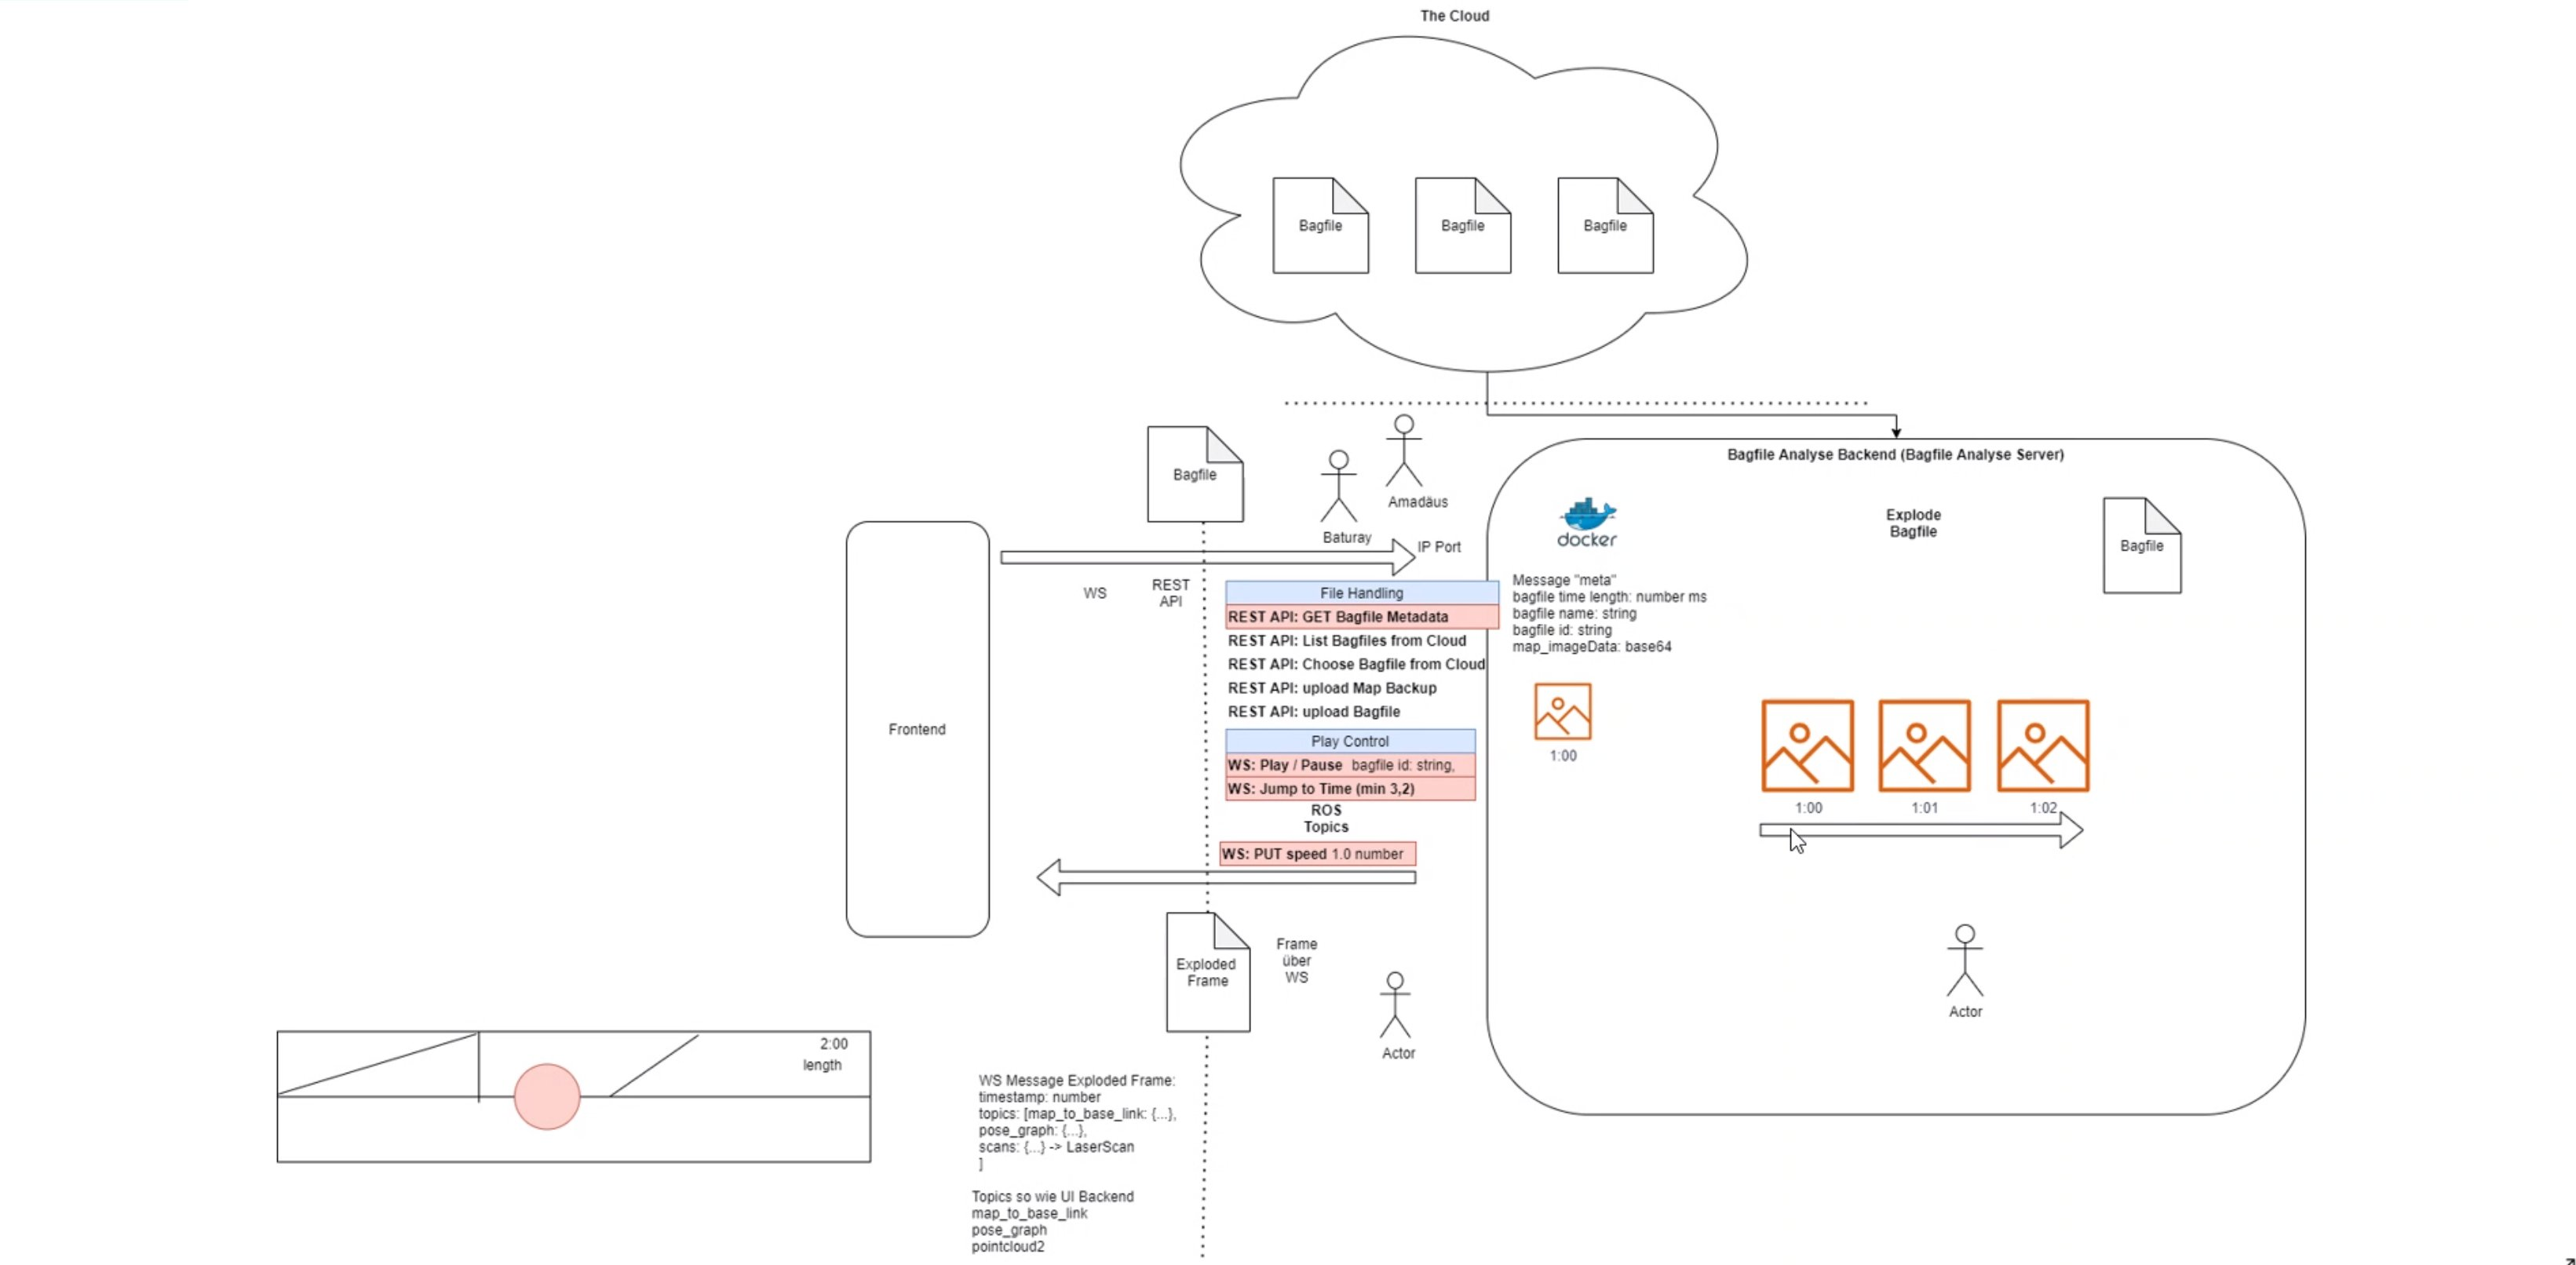
\includegraphics[height=10cm,width=\linewidth]{images/architecture.jpg}
		\caption{Architecture of Rosbag player}
	\end{center}
\end{figure}
\pagebreak
\section{Compare between different libraries}
For implementation of the backend to support rosbag play and every other functionalities python libraries must be used. There were several libraries that can be used to manipulate the rosbag on the backend. 

Basically I did research on sevaral libraries which supports the playing of the rosbag just like command ine used to play the bag.

There were many python libraries which does the same job of playing the rosbag.

\begin{enumerate}
	\item bagpy
	\item rospy
	\item rosbag
	\item pyrosbag
\end{enumerate} 
Some of the libraries which I used is as follows. There were some advantages and disadvantages of libraries.
\begin{enumerate}
	\item bagpy: This library provides a wrapper class call bagreader which is written in python. This provides an easy to use interface for reading rosbag which are recorded by rosbag record command. This library internally uses the rosbag to perform certain operations. 
	
	This library is basically used only to read the topics and there content. But this can't be used to manipulate the bag like playing, recording or anything.

	
	\item rospy: This a python client library for ROS. This client library will quickly enables to interface with ROS Topics, Services and parameters. This enables to access all the information of topics of ROS.
	
	Since we wanted to change the speed of the rosbag on the run time, so this library didn't supported in doing that. Using this library we can only change the speed of the rosbag in the starting of the bag. While running of the bag speed cannot be changed.
	
	\item rosbag: The rosbag package provides the command-line tool for working with bags as well as code APIs for writing and reading bags. This library can't be used to play the rosbag.
	
	\item pyrosbag: This is a library which will create a python library for handling of rosbag. This particular library uses the rosbag and os library to handle all the required functionalities. 
	
	Since the requirement is satisfied with this library we are using pyrosbag library in the backend to support the rosbag part.
\end{enumerate}

\section{Compare between Websockets-API and REST-API} 

In this approach, we needed the communication between the client and server, where the frontend tool will be client and backend tool will be server. So for this hybrid approach to entangle the requirements has been followed. 

\textbf{Websockets:} Websockets is bi-directional communication protocol which enables the continuous communication between the client and server. Since the playing, pausing and stopping of rosbag, stepping of rosbag must via ros-service call, so it must be continuous. Also our future goal is write as well as read ros-topic information. Since in the case of RESt-API it will create instance of that instant and it is not time efficient. Therefore the communication between the frontend and backend for the playing, increasing/decreasing, jumping to time of rosbag part is decided to be via websockets. 
 
\textbf{REST-API:} REST-API is uni-directional communication between server and client. For example in ROS-case we can only read the rostopic information, but we can write or publish to the topic. In some requirements of our project like getting list of bag-files from cloud, choosing which bagfile to be played, uploading the bagfile and uploading the map of factory, it will be one way communication. Either we write a map to cloud, or read the list of the bagfiles in cloud. So for these requirements REST-API is used for communication. 

\section{ROSBRIDGE}
In the frontend codes were implemented in JSON to create the functionalities like connecting pause and play button to the rosservices. Some other functionalities includes integration of slider with jump function.

Since the websocket interface is used for all these functionalities. So we had option of implementing with either os level program or using Rosbridge. Rosbridge provides the JSON API to ROS functionalities.Since the backend works completely with ROS, so Rosbridge is decided as API for frontend. 
 

\section{Concept to visualize the map}

As the rosbag player plays the recorded topic and actions that have been executed on factories. Before implementation of this Rosbag player UI, if the customer gives the rosbag, we will play the rosbag on rviz on our local machines with the arguement of which factories map to be displayed on the rviz background. This basically works by converting the map occupancy grid layer values into real map. Then this values are published in the \textbf{map} topic which enables the rviz to subscribe and visualize it. 

Similar idea is used in this project. So when the customer uploads the map or factory information, the occupancy grid map from backup which is updated frequently is converted to map. Then this will be published in map topic, which is subscribed by rosbridge and converted accordingly to visualize in frontend.
\section{Docker}

To make the current implementation independent of particular OS and make it independent of hardware used. Therefore everything is made compatible with Docker images and containers




